\chapter{Discussion} \label{s:discussion}

\vspace{3mm}
% \noindent\rule{17cm}{0.2pt}
\fbox {
    \parbox{\linewidth}{
      \begin{itemize}
        \item Reviewing the project aims
        \item Challenges
        \item Contribution to MIBC research
        \item Limitations
        \item Future work
      \end{itemize}
    }
}
\vspace{3mm}


\section{Meeting the aims}

This PhD project had three aims: 1) create a method that allows the integration of multiple data types, 2) use the non-tumour gene expression to inform tumour stratification, and 3) enable researchers to trace the biological mechanism behind each subtype.

% Summary of the method
The \textbf{iNet} pipeline introduced in \cref{s:N_I} and then further refined in \cref{s:N_II}, is a network approach that allows the integration of multiple data types: 1) using \textbf{edges weight} modifiers to integrate mutation burden 2) selective edge pruning, which allows \acrlong{tf} to have a higher \textbf{number of eges}, and 3) using gene expression from freshly isolated samples to build a co-expressed \textbf{network}. 

% Effects on the network show that the data was integrated successfully computationally
Throughout the thesis, the effects of the data integration were verified at the network level by analysing the changes in the network metric using different parameters for selective edge pruning or edge weight modifier strategies. It was also observed that both selective edge pruning and weight modifier influence the community detection algorithm, which in turn has an impact on the stratification of the MIBC. The co-expressed networks built from the non-tumour and tumour datasets were different in terms of network metrics, the number of communities, and the MIBC subgroups derived.

% Community detection - traceability
Community detection plays an essential role in analysing the co-expressed network as it finds groups of genes in the co-expressed networks, which are then used to stratify the MIBC. Through these communities, traceability is achieved, and it has been shown to link MIBC divisions to some of the communities, work which was covered in more detail in \cref{s:N_II:std_net}.

% 
To conclude, all three aims were tested and achieved computationally. The network method proposed allows the integration of multiple data types, enables traceability, and can be used to build the non-tumour gene expression to inform the MIBC stratification. The following sections discuss the biological implications of the work performed.

% Challengs of the work
\section{Challenges}

% Challenge of unsupervised learning
The main challenge of the project was measuring the success of the changes in computational methods which is also one of the challenges in unsupervised learning applications. The lack of ground truth characterises such applications, and not knowing what to expect from the new subgroups makes it challenging to evaluate changes in the network pipeline.

% Lack of validation from standard metrics 
To measure the impact of the changes in the network clustering metrics were used that do not require such as the Silhouette score or network metrics. These tools help verify whether modifications to the methods affect the output. However, they do not provide any indication of whether the changes made to the network have a natural biological impact. To address this, domain knowledge or further analysis was employed.

% Closest to ground truth 
The closest approximations to ground truth were the previous classifications from TCGA, Lund, and the consensus. However, it was recognised that these classifications are incomplete, as the subtypes have not yet translated into improved clinical outcomes, and they were derived only from gene expression, except for the Lund classifier, which also used \acrlong{ihc}. While these classifications served as a method to check for MIBC trends identified by various changes in the network pipeline, they fall short of providing more information when new subgroups are discovered, such as the High IFNG or Basal 5 subtypes. The only exception was the work on \acrlong{ifn} from our lab \citep{Baker2022-bj}, which, in addition to helping with MIBC splits, also provided domain knowledge that could be used to validate new groups.

% Analyses used 
An additional complexity to the analysis was added by the high heterogeneity of bladder tumour, and to validate new subtypes and understand their biological significance, methods such as \acrlong{dea}, \acrlong{gsea}, and Kaplan-Meier survival analysis were employed. The verification prorcess revealed novel biological insights and contributed with list of genes of potential markers.

In most cases, this validation process led to the discovery of new genes with the potential to reveal novel biological insights, contributing to a list of potential new markers. Additionally, the high heterogeneity of bladder tumours added to the complexity of the analysis.

% Impact of the development
In summary, measuring the success of methodological changes required extensive analysis to determine if they had a biological impact. While this process advances the understanding of bladder tissue (both cancerous and non-cancerous), it slows the development of methods and makes MIBC stratification a challenging problem to research.


% Contributon to Knowledge
\section{Advancing MIBC research}

% Basal
\subsection*{Basal and \acrlong{ifn} heterogeneity}

Using a standard clustering approach on TCGA's MIBC cohort, the research presented in \cref{s:clustering_analysis} found six subgroups, three of which were previously classified as basal and had different \acrshort{ifn} responses. Of particular interest were the Low IFNG and High IFNG, the former having a low \acrshort{ifn} and poor 5-year survival, and the latter having a high immune response with more favourable prognosis. This initial research in the project not only encouraged the later development but also highlighted that there is an understudied group of samples that can be potentially targeted by immunotherapy, which has a potential clinical impact.


% Selective edge pruning
\subsection*{Work on the \acrlong{tf}}

% Selective edge pruning
Using the selective edge pruning and the control networks, it was found that there is a subset of 98 TFs which have a strong correlation with other genes; \cref{s:N_I:sel_tfs}. Using the RNAseq data from TCGA to stratify the MIBC cohort, a new basal group, Basal 5, with less than a 20\% chance of survival after 1.7 years, this being the poorest prognosis seen in the thesis and possibly in the literature. Basal 3 was another basal group with a poor prognosis, which contained samples previously classified as Mes-like \citep{Marzouka2018-ge}.

% Basla 5
The Basal 5 subtype consists of 20 samples previously classified as basal \citep{Kamoun2020-tj,Robertson2017-mg} or UroB \citep{Marzouka2018-ge}, the latter having poor survival prognosis. It is worth noting that none of the samples in the Basal 5 were previously classified as \acrlong{ne}\footnote{\acrlong{ne} have the worst poor survival in the consensus and TCGA classifications \citep{Kamoun2020-tj,Robertson2017-mg}}. The group exhibits squamous markers and has a low immune response, and some of the significantly expressed genes are responsible for the aggressiveness of the tumours, while others can be targeted to improve treatment response.

% Selective edge pruning + controls as a method to find TFs
The biological findings indicate that the selective edge pruning and the control networks can potentially represent a new method to find relevant \acrfull{tf} in a gene expression dataset. The method can help the researchers reduce the list of potential gene regulatory networks, focusing on the co-expressed ones.

% High degree
\subsection*{Subset of genes with high degree}

The sigmoid weight modifier (or reward v2) used in the non-tumour network representation led to a selection of 122 genes with the following properties: 1) high mutation burden, 2) co-expressed with other genes, and 3) their Spearman correlation values are strong (\(>0.5\)); see \cref{s:N_II}. All the genes in this subset had a high degree value and were grouped into small-sized communities with less than 10 nodes. In addition, most genes have recognisable biological functions in the bladder, cancerous or non-cancerous.

It is remarkable that the network approach, including the \acrshort{hsbm}, can isolate genes with a functional role into small communities. An implication is that networks with more genes can be used in the network approach. This is important as gene filtering is usually required before constructing the network; thus, biases or assumptions are imposed on the network before the analysis.

% unknown genes
\subsection*{Ensembl genes}

Analysing the networks built from all the non-tumour samples showed that several communities of Ensembl genes contributed to the Abs-Ca and P0 splits, as well as to the division of TCGA's MIBC cohort. The presence of these Ensembl genes is specific to the non-tumour dataset, indicating that many poorly described genes may play an important role in bladder biology. Despite their lack of protein-coding function, recent research suggests that \acrlong{lncRNA} are implicated in gene regulatory mechanisms and chromatin remodeling \citep{Statello2021-md}, both of which are relevant to bladder cancer. This underscores the utility of a network-based approach in identifying lncRNAs, thereby imparting an additional layer of insight into bladder cancer research.

% Nework for stratifications
\subsection*{Network as a tool for MIBC subtyping}

Across the different biological processes of a tissue, the genes do not work in isolation but in relation to each other. Networks can represent this relation and even model it based on different data types. For these reasons, this project used the networks to inform the MIBC stratification. 

While there is no sufficient evidence to determine the success of the network pipeline in finding new novel MIBC subtypes, it is clear that the network representation is a useful and powerful tool for research. Through the network analysis, it was found the 98 TFs were which led to finding a subgroup of 20 samples with one of the poorest survival seen and other groups similar to the ones from Lund \citep{Marzouka2018-ge}, which were discovered using both gene expression and \acrshort{ihc} data. Using the sigmoid reward modifier, the network pipeline selected a subset of 122 genes with important molecular features (high, strong correlation and mutated) and various roles in the bladder.

The network approach suffered from a few limitations, which are addressed below. Addressing them will be part of future work to refine the methods.


% Limitations
\section{Limitations} \label{s:limitations}

% Datasets
\subsection*{Datasets}

The TCGA and non-tumour datasets are invaluable assets to bladder research, but both samples have some aspects that need consideration. The MIBC cohort from TCGA is compromised of biopsies that are considered to be predominantly aggressive forms of MIBC and come mostly from males (\(\sim74\%\)). and are predominently white (\(\sim80\%\)).

% Talk
The samples from the non-tumour datasets consist mostly of tissues from female donors (\(\sim90\%\)), and some of them are even paediatric. In the analysis performed, no biological sex difference was observed, not even in one of the Abs-Ca or P0 splits, and the predominantly female samples might impact TCGA's MIBC cohort, which is a male-dominated dataset.

Another difference between the two datasets is that the stroma cells are removed in the non-tumour samples to form a cleaner representation of the bladder tissue. In addition, the samples from the non-tumour dataset do not exhibit \acrfull{ifn} response. However, among the previous MIBC stratification, the stroma infiltration characterises groups or, as it was shown \acrshort{ifn} response. This means that the non-tumour network representation cannot find stroma-like MIBC or high immune infiltration subgroups.


\subsection*{ModCon and MEV}

One limitation of the network approach is that ModCon does not account for community size imbalance. This issue was most noticeable in the MIBC subtypes derived from the network, where there are small communities of highly connected nodes; see \cref{s:N_II:high_conn}. ModCon selects 100 genes regardless of the community size, and the MEV score is calculated as the sum of the z-scores of the genes selected by ModCon.

% Implications
When a community size is less than 100 nodes, the MEV score of the smaller community (\(<100\) nodes) is inherently smaller than that of larger communities. Consequently, smaller communities containing important genes may have a lesser impact on the MIBC stratification.


\subsection*{Basal predominant novelty} \label{s:discussion:gene_filt}

% basal the most disrupted
Finding subgroups within samples previously classified as the basal group is a recurring outcome in the analyses conducted throughout this project. One possible explanation is that basal tissues are more similar to undifferentiated bladder tissue, making them more distinct than luminal-type samples, closer to fully differentiated bladder tissue. Consequently, when the non-tumour network is used to stratify MIBC, the basal samples' most notable changes (or variations) occur. While this explanation might account for the patterns observed in the network representations, it does not apply to the clustering analysis, where \acrshort{ifn} heterogeneity was found across the basal subtypes.

% Gene filtering
The aggressive gene filtering to remove the unexpressed genes from the dataset might be another possible reason for the basal bias. With aggressive filtering, a gene is considered expressed if it is present in 90\% of the samples; in other words, any gene is discarded if it is \textbf{not} expressed in 10\% (i.e. four samples for TCGA) of the cohort. The permissive filter does the opposite; it considers unexpressed genes when it is not found in 90\% of the cohort or in 367 samples. 

Permissive filtering is more used in this field as it keeps the genes with a high variance. However, as this project showed, using an aggressive gene filtering leads to new Basal divisions that were previously found by using \acrshort{ihc} data in Lund cohort \citep{Marzouka2018-ge} or focused studies on the \acrshort{ifn} response in urothelium.

The MIBC patients are treated using BCG vaccines and can induce an \acrshort{ifn} response \citep{Baker2022-bj}. The genes ' variance is relatively low since the immune response is present in a large portion of the basal samples (i.e., High and Med IFNG). When using a permissive gene filtering approach, the \acrshort{ifn} gene signature dominates the most varied genes. However, with aggressive gene filtering, which imposes strict limits on gene expression, these highly varied genes selected through permissive filtering are excluded. As a result, this filtering method reveals the \acrlong{ifn} gamma response, which shows the rank comparison of the two filtering strategies in \cref{fig:ifng_rank_genes}.

% Implication of the finding
Finding the \acrlong{ifn} gene signature in the higher ranks of the aggressive filtering but not in the permissive filtering indicates that both approaches reveal different aspects of the same dataset. The permissive strategy promotes genes with high variance, potentially leading to subgroups with significantly different expression patterns. In contrast, aggressive gene filtering promotes gene signatures that are consistently expressed in a larger group of samples and exhibit less variation across the entire cohort.


\begin{figure}[!htb]
    \centering
    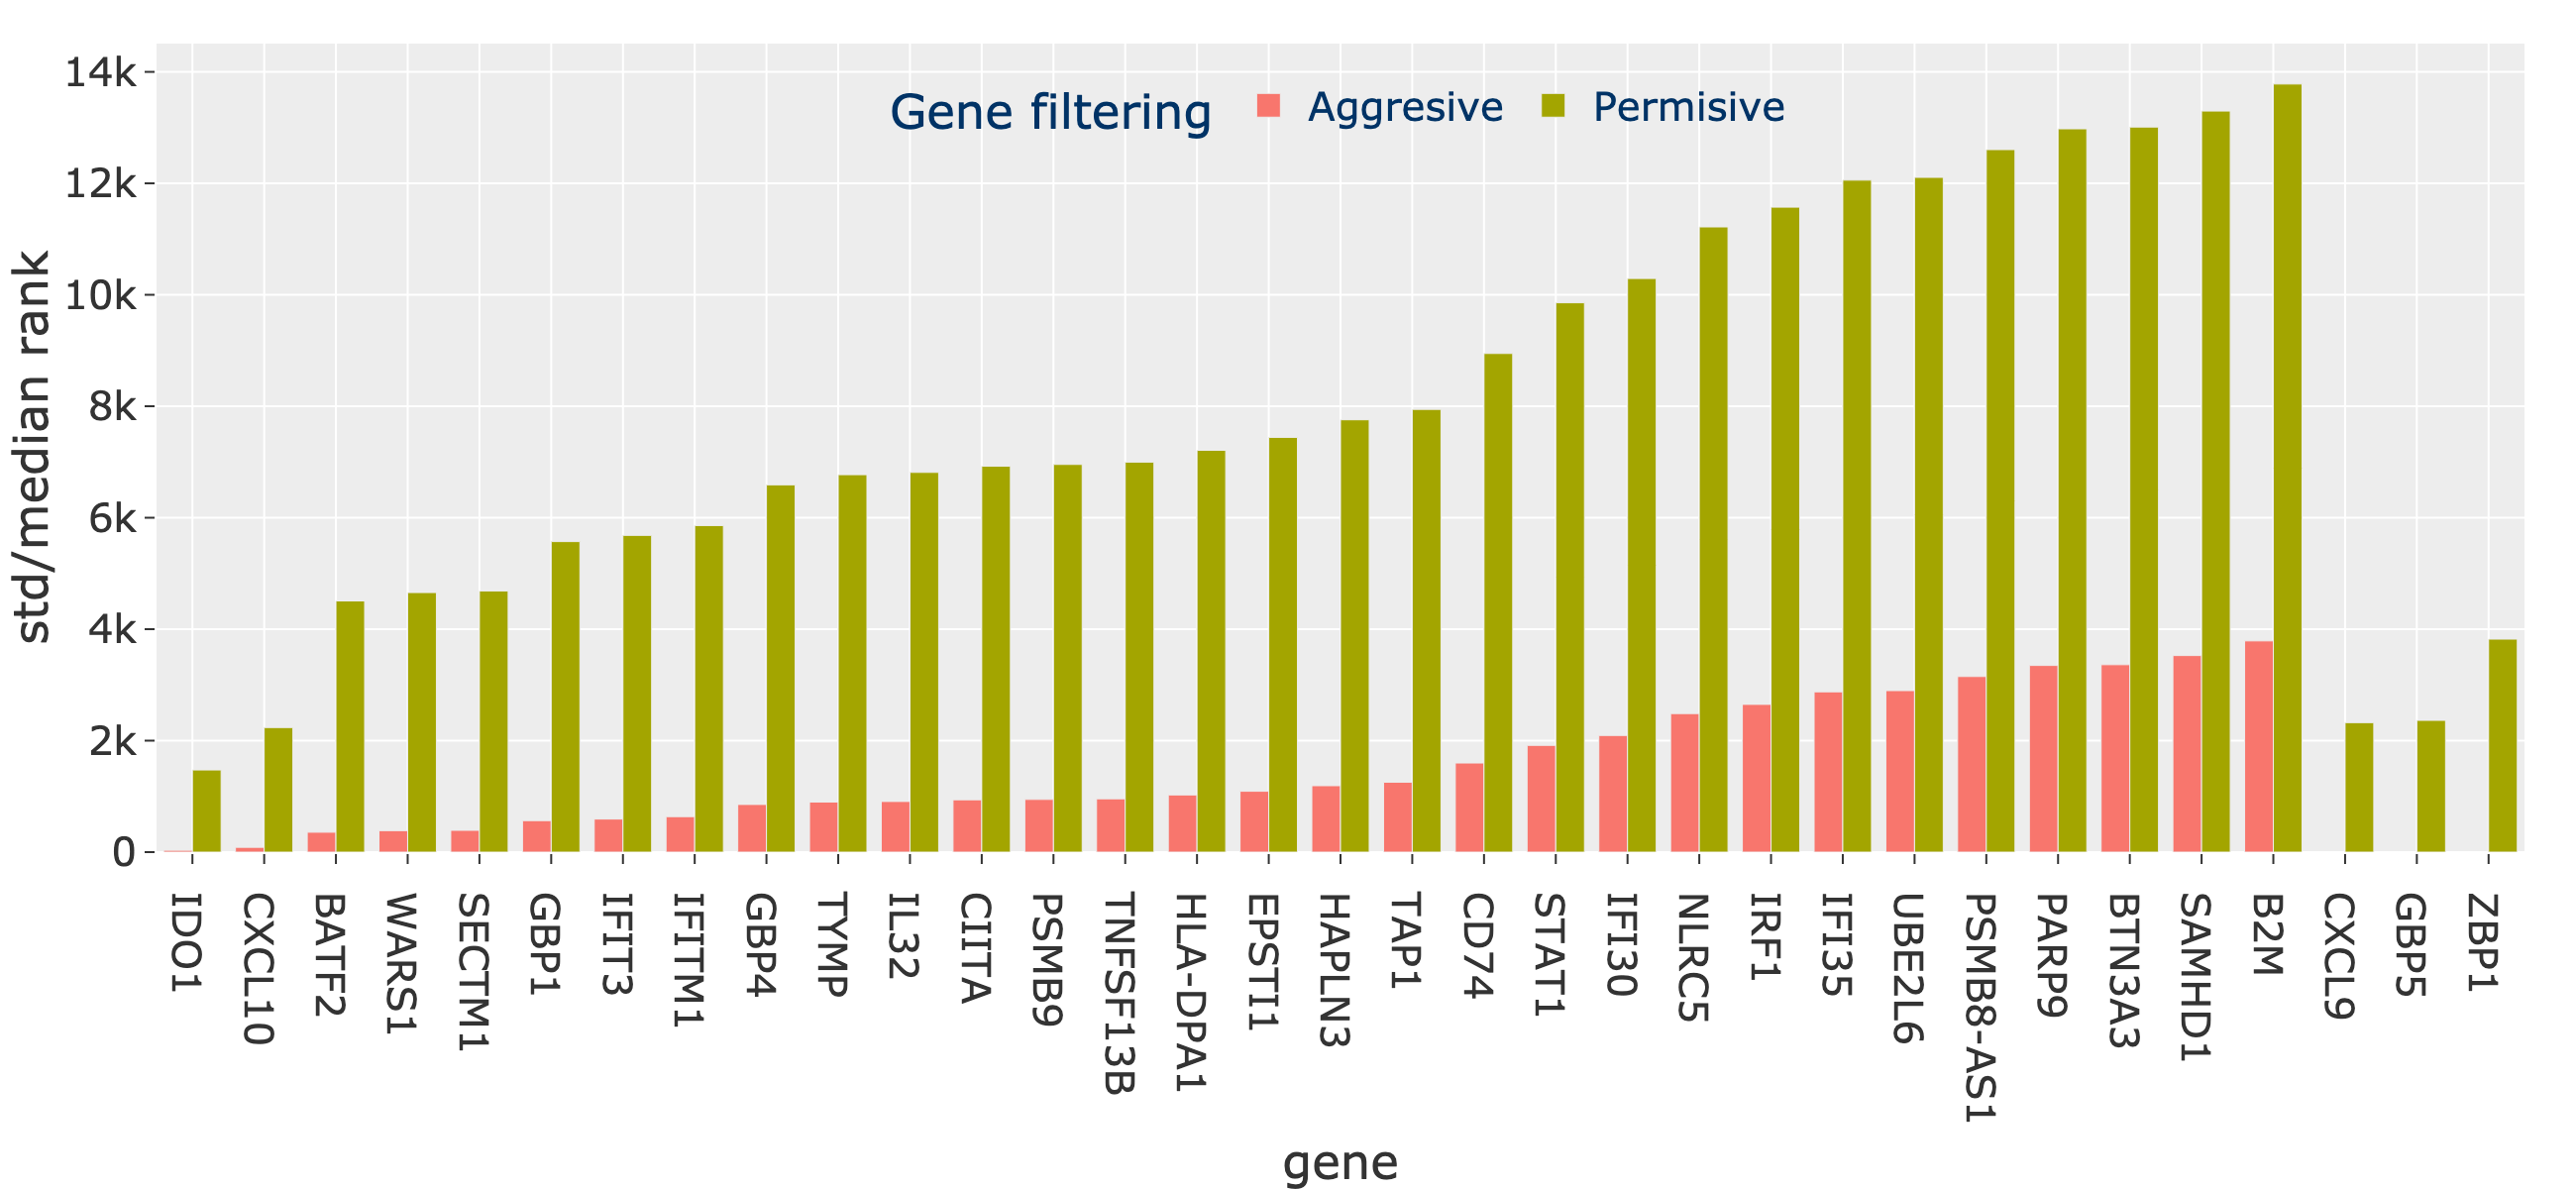
\includegraphics[width=1.0\textwidth,keepaspectratio]{Sections/Gene_Sel/ifng_ranks.png}
    \caption[Std/median ranks of the genes in \acrlong{ifn} signature]{The \acrshort{ifn} gene signature \citep{Baker2022-bj} ranked by standard deviation and median in two processed datasets. The first dataset is processed using permissive gene filtering, while the second uses aggressive gene filtering. The bar plot demonstrates that the gene signature is 'hidden' in lower ranks when applying permissive strategy, whereas the aggressive filtering reveals the \acrshort{ifn} gene signature.}
      \label{fig:ifng_rank_genes}
\end{figure}

\subsection*{Building co-expressed networks}

As mentioned in the previous section, aggressive gene filtering identified basal groups with \acrshort{ifn} heterogeneous responses. This indicates that choosing which genes to include in a network has a \textbf{substantial} impact on the subsequent MIBC stratification stage.

Aggressive gene filtering might be more appropriate for constructing a non-tumour network representation, which is then used to stratify the MIBC. Selecting genes expressed in at least 90\% of the non-tumour samples ensures that the genes forming the 'core' of the urothelium are utilised to inform cancer subtyping. This is particularly crucial when integrating the mutation burden, as the gene selection process focuses on disruptions in the co-expression of core genes expressed in the bladder.

% Discussing the potential of using more genes
An adjacent finding of the refined network, which used \acrshort{hsbm}, was that the community detection algorithm could isolate 122 genes from 5000 into small groups of fewer than 10 nodes. These genes were not a computing artefact but exhibited biological properties and functions relevant to bladder cancer. This suggests that the network approach can identify small communities, indicating that more genes can be incorporated into the network. Consequently, the initial assumptions regarding gene filtering can be relaxed, potentially leading to better data representation.

Another limitation of the co-expressed network built in this project is that only positive correlations are utilised. This means the network pipeline is constrained to identifying co-expressed genes without capturing downregulated mechanisms. To address this, separate networks can be created where the sign of the Spearman correlation values is inverted, thereby avoiding the challenges associated with using negative weights in a network—since some algorithms do not perform well with negative edge weights.


% Future work
\section{Future work} \label{s:future_work}

Due to the limited time in a PhD project and the unsupervised nature of MIBC subtyping, several areas and limitations could be improved upon and suggested for future work.

\subsection*{Larger Networks}

The research presented in this thesis suggested that the network approach could handle larger datasets, allowing for a relaxation of the assumptions about the data included in the network approach. The advantage of not imposing stringent filtering is that it reduces the likelihood of missing important genes. For example, work in the JBU lab identified \textit{RARG} as playing a substantial role in tissue differentiation, but it was ranked around the mid-5000s in the gene selection used throughout the project.

A less restrictive input dataset, such as one comprising 7,500 to 10,000 genes, could be employed in the next iteration of the network pipeline.

\subsection*{Higher Mutation Resolution}

Throughout the project, mutation burden was used to indicate the anomalies affecting genes across the MIBC cohort. However, this approach oversimplifies the complexity of mutations, as additional information is available, such as the mutation type—frame-shift, nonsense, missense, etc. Additionally, other research in the \acrlong{jbu} lab has observed that some mutated genes are not expressed and, therefore, may not impact the tumour tissue.

\subsection*{Addressing Community Size Imbalance}

The community size imbalance impacts gene selection through ModCon and indirectly affects the iMEV scores used to stratify the MIBC. This issue can be addressed by selecting a proportional number of genes relative to the community size or employing a normalisation strategy. Another improvement needed for iMEV is to account for the mutation count of each gene in each sample and the type of mutation.

\subsection*{Gene Filtering Strategies}

This chapter presented a detailed analysis of the effects of two gene filtering strategies and posited that both have merits in uncovering new biology. Therefore, it is necessary to understand better their impact on MIBC stratification and the network approach, particularly concerning graph metrics and community detection methods.

\subsection*{Alternative Correlation Measures}

Other correlation measures in the literature may offer improvements to the network representation. For example, partial correlation removes the influence of other variables on the compared pair, resulting in a 'purer' correlation value. Combining this with selective edge pruning may refine the edges retained for building the network.

\subsection*{Beyond mutations and TFs}

The project used mutation burden and TFs to model the number of edges and their strength of a node. These data types were chosen for their availability and their importance to bladder cancer, but other data types can be integrated. Disruption in the epigenetic mechanism is another molecular characteristic of bladder cancer which could be integrated into a network by adapting the reward modifiers to include data from ATAC-seq.

\subsection*{Software and Other Applications}

The software developed in this project was designed from the outset to apply to other diseases. One of the next steps will be to test it on other gene expression datasets to evaluate the method and the software package.

% Final remakrs
% \section{Final remarks}

% One essential research question lurking around all the work presented in the thesis is what is a data representation that is close to the molecular representation found in a tissue? Networks represented the natural candidate as the gene relation can be aproximated extracted correlation valeus and these links can be then modeled to reflect other dataypes.
 
% \acrlong{mibc} has a large impact on the quality of life of the patients and their close circel as well as to the healthcare sysem. This makes it imperative to study and unerstand more the disease, and one strategy is to divide the cancer into multiple groups for which targeted treatments can be developed. There has been previous research efforts to finding new subtypes with some being in clinical trials. However, these suffer from limitations which this project attempted to address by integrating multiple data types into a network representation.
